\chapter{路径与回路}

本章关注图中的两类路径：
\begin{itemize}
\item \key{欧拉路径}是一条恰好经过每条边一次的路径。
\item \key{哈密顿路径}是一条恰好访问每个节点一次的路径。
\end{itemize}

虽然欧拉路径和哈密顿路径乍看之下是相似的概念，
但与它们相关的计算问题却大不相同。
事实证明，存在一个简单的规则可以判定一个图是否包含欧拉路径，
并且如果存在这样的路径，也有高效的算法来找到它。
相反，判定哈密顿路径是否存在是一个NP困难问题，
目前没有已知的高效算法来求解该问题。

\section{欧拉路径}

\index{欧拉路径}

\key{欧拉路径}\footnote{L. Euler 在1736年解决了著名的哥尼斯堡七桥问题时研究了此类路径。
这标志着图论的诞生。}是一条恰好经过图中每条边一次的路径。
例如，以下图
\begin{center}
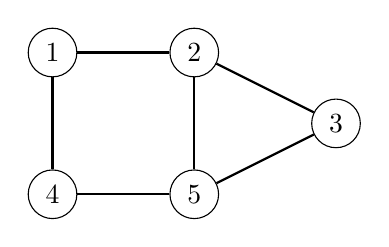
\begin{tikzpicture}[scale=0.9]
\node[draw, circle] (1) at (1,5) {$1$};
\node[draw, circle] (2) at (3,5) {$2$};
\node[draw, circle] (3) at (5,4) {$3$};
\node[draw, circle] (4) at (1,3) {$4$};
\node[draw, circle] (5) at (3,3) {$5$};

\path[draw,thick,-] (1) -- (2);
\path[draw,thick,-] (2) -- (3);
\path[draw,thick,-] (1) -- (4);
\path[draw,thick,-] (3) -- (5);
\path[draw,thick,-] (2) -- (5);
\path[draw,thick,-] (4) -- (5);
\end{tikzpicture}
\end{center}
有一条从节点2到节点5的欧拉路径：
\begin{center}
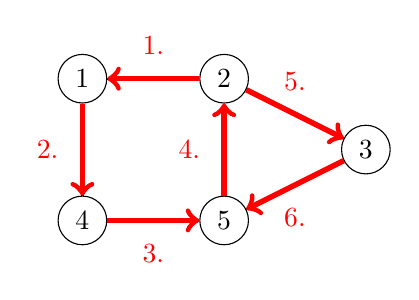
\begin{tikzpicture}[scale=0.9]
\node[draw, circle] (1) at (1,5) {$1$};
\node[draw, circle] (2) at (3,5) {$2$};
\node[draw, circle] (3) at (5,4) {$3$};
\node[draw, circle] (4) at (1,3) {$4$};
\node[draw, circle] (5) at (3,3) {$5$};

\path[draw,thick,-] (1) -- (2);
\path[draw,thick,-] (2) -- (3);
\path[draw,thick,-] (1) -- (4);
\path[draw,thick,-] (3) -- (5);
\path[draw,thick,-] (2) -- (5);
\path[draw,thick,-] (4) -- (5);

\path[draw=red,thick,->,line width=2pt] (2) -- node[font=\small,label={[red]north:1.}] {} (1);
\path[draw=red,thick,->,line width=2pt] (1) -- node[font=\small,label={[red]left:2.}] {} (4);
\path[draw=red,thick,->,line width=2pt] (4) -- node[font=\small,label={[red]south:3.}] {} (5);
\path[draw=red,thick,->,line width=2pt] (5) -- node[font=\small,label={[red]left:4.}] {} (2);
\path[draw=red,thick,->,line width=2pt] (2) -- node[font=\small,label={[red]north:5.}] {} (3);
\path[draw=red,thick,->,line width=2pt] (3) -- node[font=\small,label={[red]south:6.}] {} (5);
\end{tikzpicture}
\end{center}
\index{欧拉回路}
\key{欧拉回路}是一条起点和终点为同一节点的欧拉路径。
例如，以下图
\begin{center}
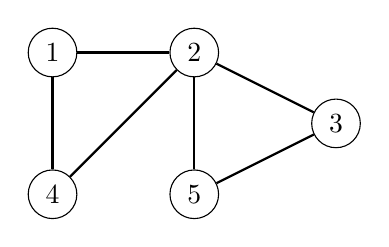
\begin{tikzpicture}[scale=0.9]
\node[draw, circle] (1) at (1,5) {$1$};
\node[draw, circle] (2) at (3,5) {$2$};
\node[draw, circle] (3) at (5,4) {$3$};
\node[draw, circle] (4) at (1,3) {$4$};
\node[draw, circle] (5) at (3,3) {$5$};

\path[draw,thick,-] (1) -- (2);
\path[draw,thick,-] (2) -- (3);
\path[draw,thick,-] (1) -- (4);
\path[draw,thick,-] (3) -- (5);
\path[draw,thick,-] (2) -- (5);
\path[draw,thick,-] (2) -- (4);
\end{tikzpicture}
\end{center}
有一条从节点1出发并回到节点1的欧拉回路：
\begin{center}
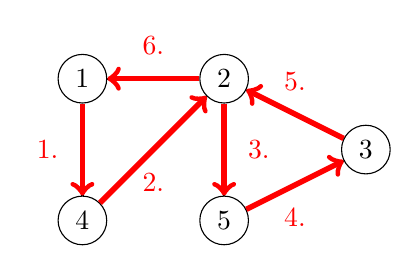
\begin{tikzpicture}[scale=0.9]
\node[draw, circle] (1) at (1,5) {$1$};
\node[draw, circle] (2) at (3,5) {$2$};
\node[draw, circle] (3) at (5,4) {$3$};
\node[draw, circle] (4) at (1,3) {$4$};
\node[draw, circle] (5) at (3,3) {$5$};

\path[draw,thick,-] (1) -- (2);
\path[draw,thick,-] (2) -- (3);
\path[draw,thick,-] (1) -- (4);
\path[draw,thick,-] (3) -- (5);
\path[draw,thick,-] (2) -- (5);
\path[draw,thick,-] (2) -- (4);

\path[draw=red,thick,->,line width=2pt] (1) -- node[font=\small,label={[red]left:1.}] {} (4);
\path[draw=red,thick,->,line width=2pt] (4) -- node[font=\small,label={[red]south:2.}] {} (2);
\path[draw=red,thick,->,line width=2pt] (2) -- node[font=\small,label={[red]right:3.}] {} (5);
\path[draw=red,thick,->,line width=2pt] (5) -- node[font=\small,label={[red]south:4.}] {} (3);
\path[draw=red,thick,->,line width=2pt] (3) -- node[font=\small,label={[red]north:5.}] {} (2);
\path[draw=red,thick,->,line width=2pt] (2) -- node[font=\small,label={[red]north:6.}] {} (1);
\end{tikzpicture}
\end{center}

\subsubsection{存在性}

欧拉路径和回路的存在性取决于节点的度数。
首先，一个无向图恰有欧拉路径的条件是所有边
属于同一个连通分量，并且
\begin{itemize}
\item 每个节点的度数都是偶数，\emph{或者}
\item 恰好有两个节点的度数是奇数，
而所有其他节点的度数都是偶数。
\end{itemize}

在第一种情况下，每条欧拉路径也是欧拉回路。
在第二种情况下，奇数度数的节点是非回路的欧拉路径的起点和终点。

\begin{samepage}
例如，在以下图中
\begin{center}
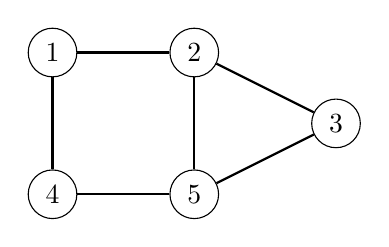
\begin{tikzpicture}[scale=0.9]
\node[draw, circle] (1) at (1,5) {$1$};
\node[draw, circle] (2) at (3,5) {$2$};
\node[draw, circle] (3) at (5,4) {$3$};
\node[draw, circle] (4) at (1,3) {$4$};
\node[draw, circle] (5) at (3,3) {$5$};

\path[draw,thick,-] (1) -- (2);
\path[draw,thick,-] (2) -- (3);
\path[draw,thick,-] (1) -- (4);
\path[draw,thick,-] (3) -- (5);
\path[draw,thick,-] (2) -- (5);
\path[draw,thick,-] (4) -- (5);
\end{tikzpicture}
\end{center}
\end{samepage}
节点1、3和4的度数为2，
节点2和5的度数为3。
恰好有两个节点的度数为奇数，
因此在节点2和节点5之间存在欧拉路径，
但该图不包含欧拉回路。

在有向图中，我们关注节点的入度和出度。
有向图恰有欧拉路径的条件是所有边属于同一个
连通分量，并且
\begin{itemize}
\item 在每个节点中，入度等于出度，\emph{或者}
\item 在一个节点中，入度比出度大1，
在另一个节点中，出度比入度大1，
而在所有其他节点中，入度等于出度。
\end{itemize}

在第一种情况下，每条欧拉路径也是欧拉回路，
在第二种情况下，图包含一条欧拉路径，
从出度较大的节点出发，到入度较大的节点结束。

例如，在以下图中
\begin{center}
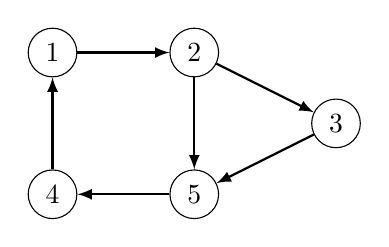
\begin{tikzpicture}[scale=0.9]
\node[draw, circle] (1) at (1,5) {$1$};
\node[draw, circle] (2) at (3,5) {$2$};
\node[draw, circle] (3) at (5,4) {$3$};
\node[draw, circle] (4) at (1,3) {$4$};
\node[draw, circle] (5) at (3,3) {$5$};

\path[draw,thick,->,>=latex] (1) -- (2);
\path[draw,thick,->,>=latex] (2) -- (3);
\path[draw,thick,->,>=latex] (4) -- (1);
\path[draw,thick,->,>=latex] (3) -- (5);
\path[draw,thick,->,>=latex] (2) -- (5);
\path[draw,thick,->,>=latex] (5) -- (4);
\end{tikzpicture}
\end{center}
节点1、3和4的入度和出度都为1，
节点2的入度为1、出度为2，
节点5的入度为2、出度为1。
因此，该图包含一条从节点2到节点5的欧拉路径：
\begin{center}
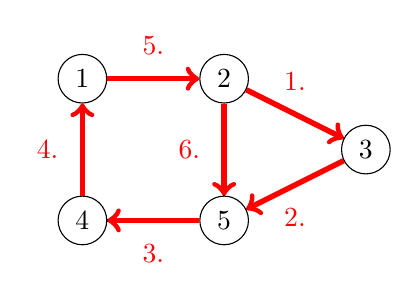
\begin{tikzpicture}[scale=0.9]
\node[draw, circle] (1) at (1,5) {$1$};
\node[draw, circle] (2) at (3,5) {$2$};
\node[draw, circle] (3) at (5,4) {$3$};
\node[draw, circle] (4) at (1,3) {$4$};
\node[draw, circle] (5) at (3,3) {$5$};

\path[draw,thick,-] (1) -- (2);
\path[draw,thick,-] (2) -- (3);
\path[draw,thick,-] (1) -- (4);
\path[draw,thick,-] (3) -- (5);
\path[draw,thick,-] (2) -- (5);
\path[draw,thick,-] (4) -- (5);

\path[draw=red,thick,->,line width=2pt] (2) -- node[font=\small,label={[red]north:1.}] {} (3);
\path[draw=red,thick,->,line width=2pt] (3) -- node[font=\small,label={[red]south:2.}] {} (5);
\path[draw=red,thick,->,line width=2pt] (5) -- node[font=\small,label={[red]south:3.}] {} (4);
\path[draw=red,thick,->,line width=2pt] (4) -- node[font=\small,label={[red]left:4.}] {} (1);
\path[draw=red,thick,->,line width=2pt] (1) -- node[font=\small,label={[red]north:5.}] {} (2);
\path[draw=red,thick,->,line width=2pt] (2) -- node[font=\small,label={[red]left:6.}] {} (5);
\end{tikzpicture}
\end{center}

\subsubsection{Hierholzer算法}

\index{Hierholzer算法}

\key{Hierholzer算法}\footnote{该算法于1873年在Hierholzer去世后发表 \cite{hie73}。}是一种构造欧拉回路的高效方法。
该算法由若干轮组成，每轮向回路中添加新的边。
当然，我们假设图中包含欧拉回路；否则Hierholzer算法无法找到它。

首先，算法构造一个包含图中部分（不一定全部）边的回路。
然后，算法通过向回路中添加子回路来逐步扩展。
该过程持续进行，直到所有边都被加入回路。

算法通过不断找到属于回路但具有不在回路中的出边的节点 $x$ 来扩展回路。
算法从节点 $x$ 出发构造一条新路径，
该路径只包含尚未在回路中的边。
迟早，
路径会回到节点 $x$，从而形成一个子回路。

如果图只包含欧拉路径（而非回路），
我们仍然可以使用Hierholzer算法来找到它，
只需在图中添加一条额外的边，
并在构造回路后移除该边。
例如，在无向图中，
我们在两个奇数度数的节点之间添加额外的边。

接下来我们将看到Hierholzer算法如何
为一个无向图构造欧拉回路。

\subsubsection{示例}

\begin{samepage}
让我们考虑以下图：
\begin{center}
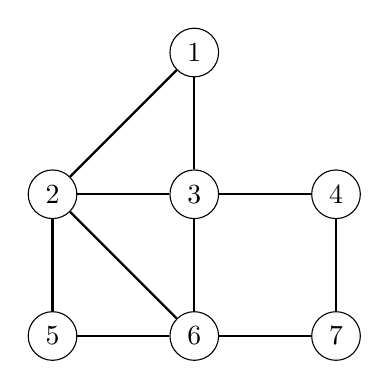
\begin{tikzpicture}[scale=0.9]
\node[draw, circle] (1) at (3,5) {$1$};
\node[draw, circle] (2) at (1,3) {$2$};
\node[draw, circle] (3) at (3,3) {$3$};
\node[draw, circle] (4) at (5,3) {$4$};
\node[draw, circle] (5) at (1,1) {$5$};
\node[draw, circle] (6) at (3,1) {$6$};
\node[draw, circle] (7) at (5,1) {$7$};

\path[draw,thick,-] (1) -- (2);
\path[draw,thick,-] (1) -- (3);
\path[draw,thick,-] (2) -- (3);
\path[draw,thick,-] (2) -- (5);
\path[draw,thick,-] (2) -- (6);
\path[draw,thick,-] (3) -- (4);
\path[draw,thick,-] (3) -- (6);
\path[draw,thick,-] (4) -- (7);
\path[draw,thick,-] (5) -- (6);
\path[draw,thick,-] (6) -- (7);
\end{tikzpicture}
\end{center}
\end{samepage}

\begin{samepage}
假设算法首先构造一个从节点1出发的回路。
一个可能的回路是
$1 \rightarrow 2 \rightarrow 3 \rightarrow 1$:
\begin{center}
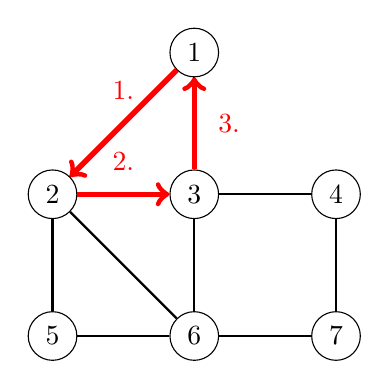
\begin{tikzpicture}[scale=0.9]
\node[draw, circle] (1) at (3,5) {$1$};
\node[draw, circle] (2) at (1,3) {$2$};
\node[draw, circle] (3) at (3,3) {$3$};
\node[draw, circle] (4) at (5,3) {$4$};
\node[draw, circle] (5) at (1,1) {$5$};
\node[draw, circle] (6) at (3,1) {$6$};
\node[draw, circle] (7) at (5,1) {$7$};

\path[draw,thick,-] (1) -- (2);
\path[draw,thick,-] (1) -- (3);
\path[draw,thick,-] (2) -- (3);
\path[draw,thick,-] (2) -- (5);
\path[draw,thick,-] (2) -- (6);
\path[draw,thick,-] (3) -- (4);
\path[draw,thick,-] (3) -- (6);
\path[draw,thick,-] (4) -- (7);
\path[draw,thick,-] (5) -- (6);
\path[draw,thick,-] (6) -- (7);

\path[draw=red,thick,->,line width=2pt] (1) -- node[font=\small,label={[red]north:1.}] {} (2);
\path[draw=red,thick,->,line width=2pt] (2) -- node[font=\small,label={[red]north:2.}] {} (3);
\path[draw=red,thick,->,line width=2pt] (3) -- node[font=\small,label={[red]east:3.}] {} (1);
\end{tikzpicture}
\end{center}
\end{samepage}
之后，算法将子回路
$2 \rightarrow 5 \rightarrow 6 \rightarrow 2$
加入回路中：
\begin{center}
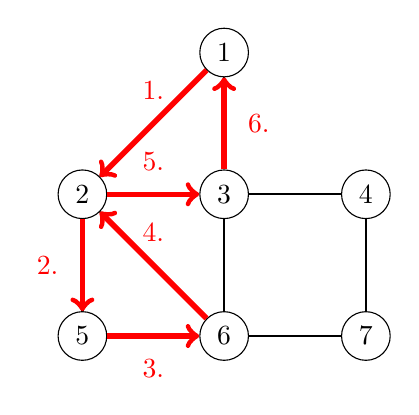
\begin{tikzpicture}[scale=0.9]
\node[draw, circle] (1) at (3,5) {$1$};
\node[draw, circle] (2) at (1,3) {$2$};
\node[draw, circle] (3) at (3,3) {$3$};
\node[draw, circle] (4) at (5,3) {$4$};
\node[draw, circle] (5) at (1,1) {$5$};
\node[draw, circle] (6) at (3,1) {$6$};
\node[draw, circle] (7) at (5,1) {$7$};

\path[draw,thick,-] (1) -- (2);
\path[draw,thick,-] (1) -- (3);
\path[draw,thick,-] (2) -- (3);
\path[draw,thick,-] (2) -- (5);
\path[draw,thick,-] (2) -- (6);
\path[draw,thick,-] (3) -- (4);
\path[draw,thick,-] (3) -- (6);
\path[draw,thick,-] (4) -- (7);
\path[draw,thick,-] (5) -- (6);
\path[draw,thick,-] (6) -- (7);

\path[draw=red,thick,->,line width=2pt] (1) -- node[font=\small,label={[red]north:1.}] {} (2);
\path[draw=red,thick,->,line width=2pt] (2) -- node[font=\small,label={[red]west:2.}] {} (5);
\path[draw=red,thick,->,line width=2pt] (5) -- node[font=\small,label={[red]south:3.}] {} (6);
\path[draw=red,thick,->,line width=2pt] (6) -- node[font=\small,label={[red]north:4.}] {} (2);
\path[draw=red,thick,->,line width=2pt] (2) -- node[font=\small,label={[red]north:5.}] {} (3);
\path[draw=red,thick,->,line width=2pt] (3) -- node[font=\small,label={[red]east:6.}] {} (1);
\end{tikzpicture}
\end{center}
最后，算法将子回路
$6 \rightarrow 3 \rightarrow 4 \rightarrow 7 \rightarrow 6$
加入回路中：
\begin{center}
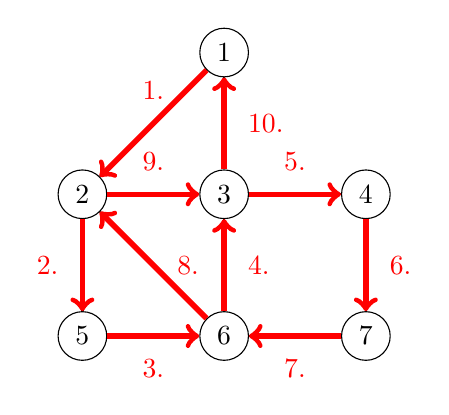
\begin{tikzpicture}[scale=0.9]
\node[draw, circle] (1) at (3,5) {$1$};
\node[draw, circle] (2) at (1,3) {$2$};
\node[draw, circle] (3) at (3,3) {$3$};
\node[draw, circle] (4) at (5,3) {$4$};
\node[draw, circle] (5) at (1,1) {$5$};
\node[draw, circle] (6) at (3,1) {$6$};
\node[draw, circle] (7) at (5,1) {$7$};

\path[draw,thick,-] (1) -- (2);
\path[draw,thick,-] (1) -- (3);
\path[draw,thick,-] (2) -- (3);
\path[draw,thick,-] (2) -- (5);
\path[draw,thick,-] (2) -- (6);
\path[draw,thick,-] (3) -- (4);
\path[draw,thick,-] (3) -- (6);
\path[draw,thick,-] (4) -- (7);
\path[draw,thick,-] (5) -- (6);
\path[draw,thick,-] (6) -- (7);

\path[draw=red,thick,->,line width=2pt] (1) -- node[font=\small,label={[red]north:1.}] {} (2);
\path[draw=red,thick,->,line width=2pt] (2) -- node[font=\small,label={[red]west:2.}] {} (5);
\path[draw=red,thick,->,line width=2pt] (5) -- node[font=\small,label={[red]south:3.}] {} (6);
\path[draw=red,thick,->,line width=2pt] (6) -- node[font=\small,label={[red]east:4.}] {} (3);
\path[draw=red,thick,->,line width=2pt] (3) -- node[font=\small,label={[red]north:5.}] {} (4);
\path[draw=red,thick,->,line width=2pt] (4) -- node[font=\small,label={[red]east:6.}] {} (7);
\path[draw=red,thick,->,line width=2pt] (7) -- node[font=\small,label={[red]south:7.}] {} (6);
\path[draw=red,thick,->,line width=2pt] (6) -- node[font=\small,label={[red]right:8.}] {} (2);
\path[draw=red,thick,->,line width=2pt] (2) -- node[font=\small,label={[red]north:9.}] {} (3);
\path[draw=red,thick,->,line width=2pt] (3) -- node[font=\small,label={[red]east:10.}] {} (1);
\end{tikzpicture}
\end{center}
现在所有边都已包含在回路中，
我们成功构造了一个欧拉回路。

\section{哈密顿路径}

\index{哈密顿路径}

\key{哈密顿路径}
%\footnote{W. R. Hamilton (1805--1865) 是一位爱尔兰数学家。}
是一条恰好访问图中每个节点一次的路径。
例如，以下图
\begin{center}
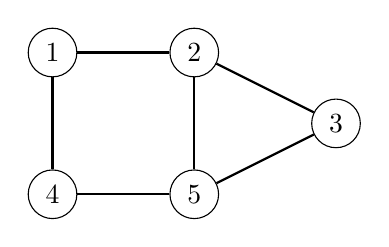
\begin{tikzpicture}[scale=0.9]
\node[draw, circle] (1) at (1,5) {$1$};
\node[draw, circle] (2) at (3,5) {$2$};
\node[draw, circle] (3) at (5,4) {$3$};
\node[draw, circle] (4) at (1,3) {$4$};
\node[draw, circle] (5) at (3,3) {$5$};

\path[draw,thick,-] (1) -- (2);
\path[draw,thick,-] (2) -- (3);
\path[draw,thick,-] (1) -- (4);
\path[draw,thick,-] (3) -- (5);
\path[draw,thick,-] (2) -- (5);
\path[draw,thick,-] (4) -- (5);
\end{tikzpicture}
\end{center}
包含一条从节点1到节点3的哈密顿路径：
\begin{center}
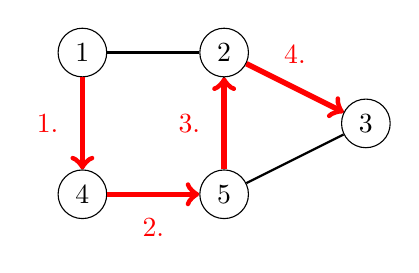
\begin{tikzpicture}[scale=0.9]
\node[draw, circle] (1) at (1,5) {$1$};
\node[draw, circle] (2) at (3,5) {$2$};
\node[draw, circle] (3) at (5,4) {$3$};
\node[draw, circle] (4) at (1,3) {$4$};
\node[draw, circle] (5) at (3,3) {$5$};

\path[draw,thick,-] (1) -- (2);
\path[draw,thick,-] (2) -- (3);
\path[draw,thick,-] (1) -- (4);
\path[draw,thick,-] (3) -- (5);
\path[draw,thick,-] (2) -- (5);
\path[draw,thick,-] (4) -- (5);

\path[draw=red,thick,->,line width=2pt] (1) -- node[font=\small,label={[red]left:1.}] {} (4);
\path[draw=red,thick,->,line width=2pt] (4) -- node[font=\small,label={[red]south:2.}] {} (5);
\path[draw=red,thick,->,line width=2pt] (5) -- node[font=\small,label={[red]left:3.}] {} (2);
\path[draw=red,thick,->,line width=2pt] (2) -- node[font=\small,label={[red]north:4.}] {} (3);
\end{tikzpicture}
\end{center}

\index{哈密顿回路}

如果一条哈密顿路径的起点和终点是同一个节点，
则称为\key{哈密顿回路}。
上面的图也有一条从节点1出发并回到节点1的哈密顿回路：
\begin{center}
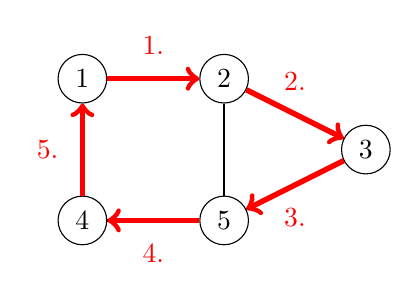
\begin{tikzpicture}[scale=0.9]
\node[draw, circle] (1) at (1,5) {$1$};
\node[draw, circle] (2) at (3,5) {$2$};
\node[draw, circle] (3) at (5,4) {$3$};
\node[draw, circle] (4) at (1,3) {$4$};
\node[draw, circle] (5) at (3,3) {$5$};

\path[draw,thick,-] (1) -- (2);
\path[draw,thick,-] (2) -- (3);
\path[draw,thick,-] (1) -- (4);
\path[draw,thick,-] (3) -- (5);
\path[draw,thick,-] (2) -- (5);
\path[draw,thick,-] (4) -- (5);

\path[draw=red,thick,->,line width=2pt] (1) -- node[font=\small,label={[red]north:1.}] {} (2);
\path[draw=red,thick,->,line width=2pt] (2) -- node[font=\small,label={[red]north:2.}] {} (3);
\path[draw=red,thick,->,line width=2pt] (3) -- node[font=\small,label={[red]south:3.}] {} (5);
\path[draw=red,thick,->,line width=2pt] (5) -- node[font=\small,label={[red]south:4.}] {} (4);
\path[draw=red,thick,->,line width=2pt] (4) -- node[font=\small,label={[red]left:5.}] {} (1);
\end{tikzpicture}
\end{center}

\subsubsection{存在性}

目前没有已知的高效方法来检测一个图是否包含哈密顿路径，
该问题是NP困难的。
尽管如此，在一些特殊情况下，
我们可以确定一个图包含哈密顿路径。

一个简单的观察是，如果图是完全图，
即每对节点之间都有一条边，
则它也包含哈密顿路径。
还有更强的结论：

\begin{itemize}
\item
\index{Dirac定理}
\key{Dirac定理}： %\cite{dir52}
如果每个节点的度数至少为 $n/2$，
则图包含哈密顿路径。
\item
\index{Ore定理}
\key{Ore定理}： %\cite{ore60}
如果每对不相邻节点的度数之和
至少为 $n$，
则图包含哈密顿路径。
\end{itemize}

这些定理和其他结论的共同特征是，
当图有\emph{大量}边时，它们保证了哈密顿路径的存在。
这是合理的，因为图中的边越多，
构造哈密顿路径的可能性就越大。

\subsubsection{构造}

由于没有高效的方法来检查哈密顿路径是否存在，
显然也没有高效构造该路径的方法，
否则我们可以直接尝试构造路径并查看其是否存在。

一种简单的哈密顿路径搜索方法是使用回溯算法，
遍历所有可能的路径构造方式。
该算法的时间复杂度至少为 $O(n!)$，
因为有 $n!$ 种不同的 $n$ 个节点的排列顺序。

更高效的解决方案基于动态规划
（参见第10.5章）。
其思想是计算函数
$\texttt{possible}(S,x)$ 的值，
其中 $S$ 是节点的子集，$x$ 是其中一个节点。
该函数指示是否存在一条哈密顿路径
访问 $S$ 的所有节点并结束于节点 $x$。
该解决方案可以在 $O(2^n n^2)$ 时间内实现。

\section{德布鲁因序列}

\index{德布鲁因序列}

\key{德布鲁因序列}
是一个字符串，对于固定的包含 $k$ 个字符的字母表，
它恰好将每个长度为 $n$ 的字符串作为子串包含一次。
这样的字符串长度为
$k^n+n-1$ 个字符。
例如，当 $n=3$ 且 $k=2$ 时，
一个德布鲁因序列的例子是
\[0001011100.\]
该字符串的子串包含了三位二进制数的所有组合：
000、001、010、011、100、101、110 和 111。

事实上，每个德布鲁因序列对应图中的一条欧拉路径。
其思想是构造一个图，其中每个节点包含一个 $n-1$ 个字符的字符串，
每条边向字符串中添加一个字符。
以下图对应上述场景：

\begin{center}
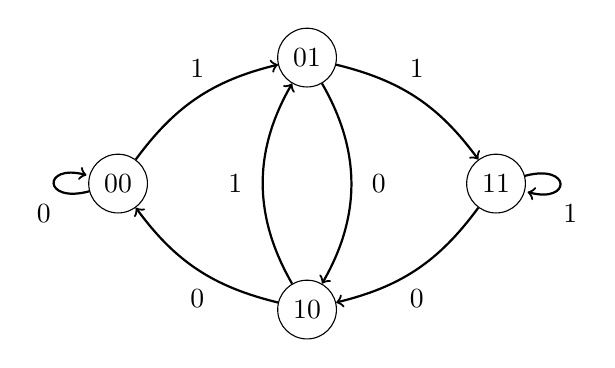
\begin{tikzpicture}[scale=0.8]
\node[draw, circle] (00) at (-3,0) {00};
\node[draw, circle] (11) at (3,0) {11};
\node[draw, circle] (01) at (0,2) {01};
\node[draw, circle] (10) at (0,-2) {10};

\path[draw,thick,->] (00) edge [bend left=20] node[font=\small,label=1] {} (01);
\path[draw,thick,->] (01) edge [bend left=20] node[font=\small,label=1] {} (11);
\path[draw,thick,->] (11) edge [bend left=20] node[font=\small,label=below:0] {} (10);
\path[draw,thick,->] (10) edge [bend left=20] node[font=\small,label=below:0] {} (00);

\path[draw,thick,->] (01) edge [bend left=30] node[font=\small,label=right:0] {} (10);
\path[draw,thick,->] (10) edge [bend left=30] node[font=\small,label=left:1] {} (01);

\path[draw,thick,-] (00) edge [loop left] node[font=\small,label=below:0] {} (00);
\path[draw,thick,-] (11) edge [loop right] node[font=\small,label=below:1] {} (11);
\end{tikzpicture}
\end{center}

该图中的欧拉路径对应一个包含所有长度为 $n$ 的字符串的字符串。
该字符串包含起始节点的字符和所有边的字符。
起始节点有 $n-1$ 个字符，
边共有 $k^n$ 个字符，
因此字符串的长度为 $k^n+n-1$。

\section{马步遍历}

\index{马步遍历}

\key{马步遍历}是马在 $n \times n$ 棋盘上
按照国际象棋规则的一系列移动，
使得马恰好访问每个格子一次。
如果马最终回到起始格子，则称为\emph{闭合}遍历，
否则称为\emph{开放}遍历。

例如，以下是在 $5 \times 5$ 棋盘上的一个开放马步遍历：

\begin{center}
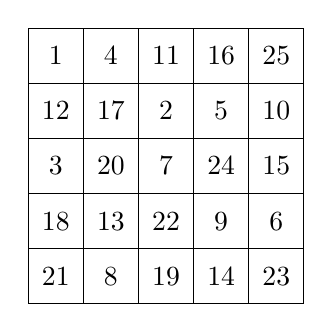
\begin{tikzpicture}[scale=0.7]
\draw (0,0) grid (5,5);
\node at (0.5,4.5) {$1$};
\node at (1.5,4.5) {$4$};
\node at (2.5,4.5) {$11$};
\node at (3.5,4.5) {$16$};
\node at (4.5,4.5) {$25$};
\node at (0.5,3.5) {$12$};
\node at (1.5,3.5) {$17$};
\node at (2.5,3.5) {$2$};
\node at (3.5,3.5) {$5$};
\node at (4.5,3.5) {$10$};
\node at (0.5,2.5) {$3$};
\node at (1.5,2.5) {$20$};
\node at (2.5,2.5) {$7$};
\node at (3.5,2.5) {$24$};
\node at (4.5,2.5) {$15$};
\node at (0.5,1.5) {$18$};
\node at (1.5,1.5) {$13$};
\node at (2.5,1.5) {$22$};
\node at (3.5,1.5) {$9$};
\node at (4.5,1.5) {$6$};
\node at (0.5,0.5) {$21$};
\node at (1.5,0.5) {$8$};
\node at (2.5,0.5) {$19$};
\node at (3.5,0.5) {$14$};
\node at (4.5,0.5) {$23$};
\end{tikzpicture}
\end{center}

马步遍历对应图中的一条哈密顿路径，
其中节点代表棋盘上的格子，
如果马按照国际象棋规则可以在两个格子之间移动，
则这两个节点之间有一条边。

构造马步遍历的一种自然方法是使用回溯。
可以使用\emph{启发式}方法来提高搜索效率，
尝试引导马快速找到一个完整的遍历。

\subsubsection{Warnsdorf规则}

\index{启发式}
\index{Warnsdorf规则}

\key{Warnsdorf规则}是一种简单而有效的寻找马步遍历的启发式方法\footnote{该启发式方法于1823年在Warnsdorf的著作 \cite{war23} 中提出。
也有多项式算法可以寻找马步遍历 \cite{par97}，
但它们更为复杂。}。
使用该规则，即使在大棋盘上也能高效地构造遍历。
其思想是每次将马移动到一个格子，
使得该格子处的可能移动数尽可能\emph{小}。

例如，在以下局面中，马有五个可能的移动格子（方格 $a \ldots e$）：
\begin{center}
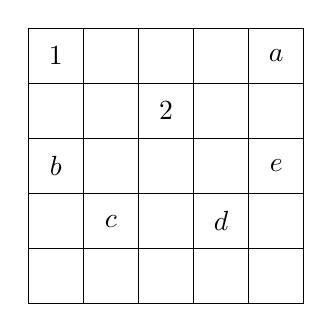
\begin{tikzpicture}[scale=0.7]
\draw (0,0) grid (5,5);
\node at (0.5,4.5) {$1$};
\node at (2.5,3.5) {$2$};
\node at (4.5,4.5) {$a$};
\node at (0.5,2.5) {$b$};
\node at (4.5,2.5) {$e$};
\node at (1.5,1.5) {$c$};
\node at (3.5,1.5) {$d$};
\end{tikzpicture}
\end{center}
在这种情况下，Warnsdorf规则将马移动到方格 $a$，
因为在此选择之后，只剩下一个可能的移动。
其他选择会将马移动到有
三个可选移动的方格。


